% !TeX root = ../main.tex

\section*{K-means}

\begin{itemize}
	\item \textbf{Initialization:} randomly assign k mean vectors as cluster centers
	\item \textbf{Repeat:}
		\begin{itemize}
			\item Assign each observation to the closest cluster mean
			\item For a given cluster assignment \(C\), compute each clusters mean
		\end{itemize}
	\item \textbf{Stopping criterium:} no more change between iterations or number of iterations exceeded.
\end{itemize}

Each iteration reduces the value of the criterion, so that convergence is assured, but the solution may be local minimum depending on the initial (random) assignment\footnote{practical approach: apply k-means multiple times (with random initialization) and choose best result.}. In addition, on should start the algorithm with many different random choices for the starting means, and choose the solution having smallest value of the objective function.

As a quality measure we use the within-cluster scatter, which can be written as
\begin{equation*}
	W(C) = \sum_{k=1}^K N_k \sum_{C(i) = k} ||x_i - \mu_k||^2
\end{equation*}
where \(\mu_k\) is the mean vector associated with the \(k\)th cluster, and \(N_k\) is the number of observations assigned to a cluster. K must be chosen beforehand. Thus, the criterion is minimized by assigning the \(N\) observations to the \(K\) clusters in such a way that within each cluster the average dissimilarity of the observations from the cluster mean, as defined by the points in that cluster, is minimized.

\subsection*{Vector Quantization}
The \(K\)-means clustering algorithm represents a key tool in the apparently unrelated area of image and signal compression, particular in \textit{vector quantization} or \textit{VQ}(Gersho and Gray, 1992).

\textbf{Algorithm}:
\begin{enumerate}
    \item Convert to grayscale
    \item Break image into small blocks, e.g. \(2 \times 2\) blocks of pixels
    \item Each block is regarded as a vector in \(\mathcal{R}^4\)
    \item Apply \(K\)-means
    \item Each of the blocks is approximated by its closest cluster centroid, known as codeword. The clustering process is called the \textit{encoding} step, and the collection of centroids is called the \textit{codebook}.
\end{enumerate}

\subsection*{\(K\)-medoids}
 \(K-\)means struggles with outliers, because using \textit{squared} Euclidean distance places the highest influence on the larger distances.

 Instead of taking means as cluster center, one can identify the sample inside each cluster, which is nearest to all other samples inside it. One then assigns this sample to be the new cluster center.

 The downside is that \(K\)-medoids is far more computationally intensive.

\subsection*{Spectral clustering}
This is essentially executing Laplacian Eigenmaps + \(k\)-Means on the lower dimensional space.

How to choose a appropriate \(d'\)? The distribution of the eigenvalues gives an indication about the intrinsic dimensionality of the data. If there is a certain gap between eigenvalue, this is a good indication. We don't have this available when using LLE.

\subsection*{Gaussian Mixtures as Soft K-means Clustering}
The \(K\)-means clustering procedure is closely related to the EM algorithm for estimating a certain Gaussian mixture model. Suppose we specify \(K\) mixture components, each with a Gaussian density having a scalar covariance matrix \(\sigma^2 I\). Then the relative density under each mixture component is a monotone function of the Euclidean distance between the data point and the mixture center. Hence in this setup EM is a "soft" version of \(K\)-means clustering, making probabilistic assignments of points to cluster centers. As the variance \(\sigma^2 \rightarrow 0\), these probabilities become 0 and 1, and the two methods coincide (responsibility of mixture component \(i: \frac{g_i(x)}{\sum_m g_m(x)}\)).

\paragraph{Short reminder: Gaussian mixture models}

Start with random initialization, expectation (how much does each component contribute to each point), maximization (update component parameters), repeat until convergence

\begin{figure}[H]
  \centering
  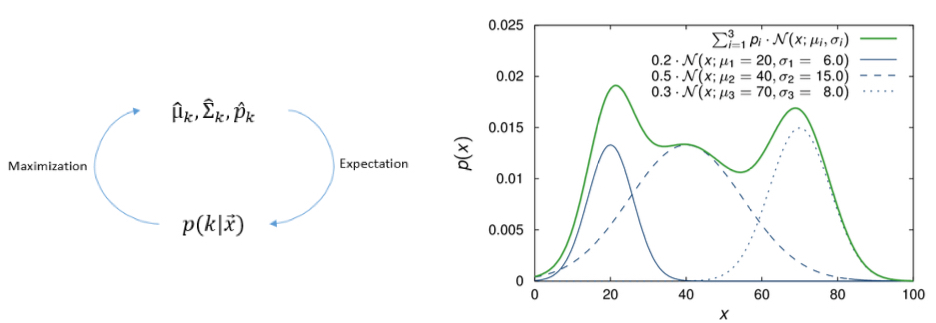
\includegraphics[width=0.7\textwidth]{GMM_EM}
\end{figure}

From a more abstract perspective, EM performs two tasks simultaneously: segmentation/clustering assignment, and model parameters estimation/fitting

 \subsection*{Practical Issues}
 In order to use \(K\)-means or -medoids one must select the number of clusters \(K^*\) as initialization. A choice for the number of clusters \(K\) depends on the goal. For data segmentation \(K\) is usually defined a part of the problem.

 Data-based methods for estimating \(K^*\) typically examine the within cluster dissimilarity \(W_k\) as a function of the number of clusters \(K\). Separate solutions are obtained for \(K \in \{1,2,\dots,K_{max}\}\). The corresponding values generally decrease with increasing \(K\).

\begin{figure}[H]
 	\centering
 	\begin{minipage}[b]{0.49\textwidth}
   	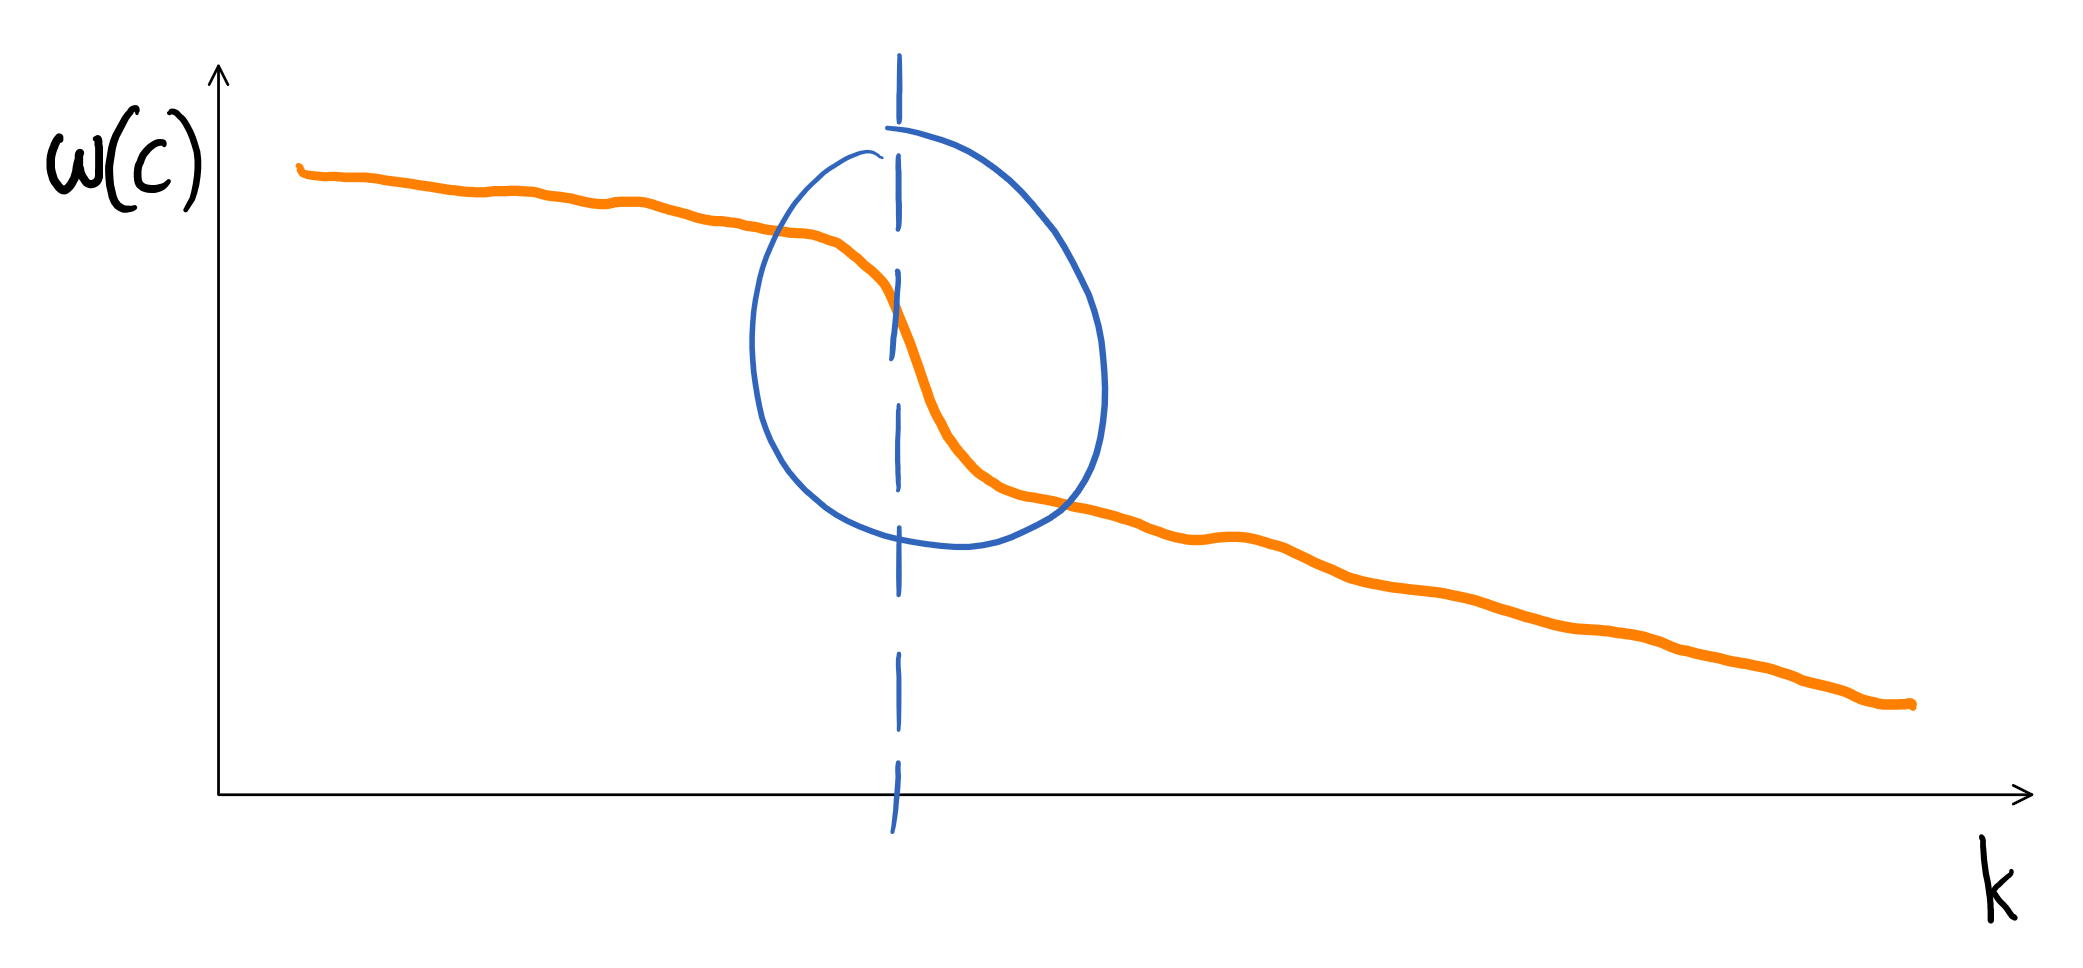
\includegraphics[width=\textwidth]{07-rate-of-change}
   \caption{Approach 1: Track the rate of change of a quality metric (like $w(c)$). Proposed in ``Pattern Classification'' (Duda, Hart, Stork).}
 	\end{minipage}
 	\begin{minipage}[b]{0.49\textwidth}
   	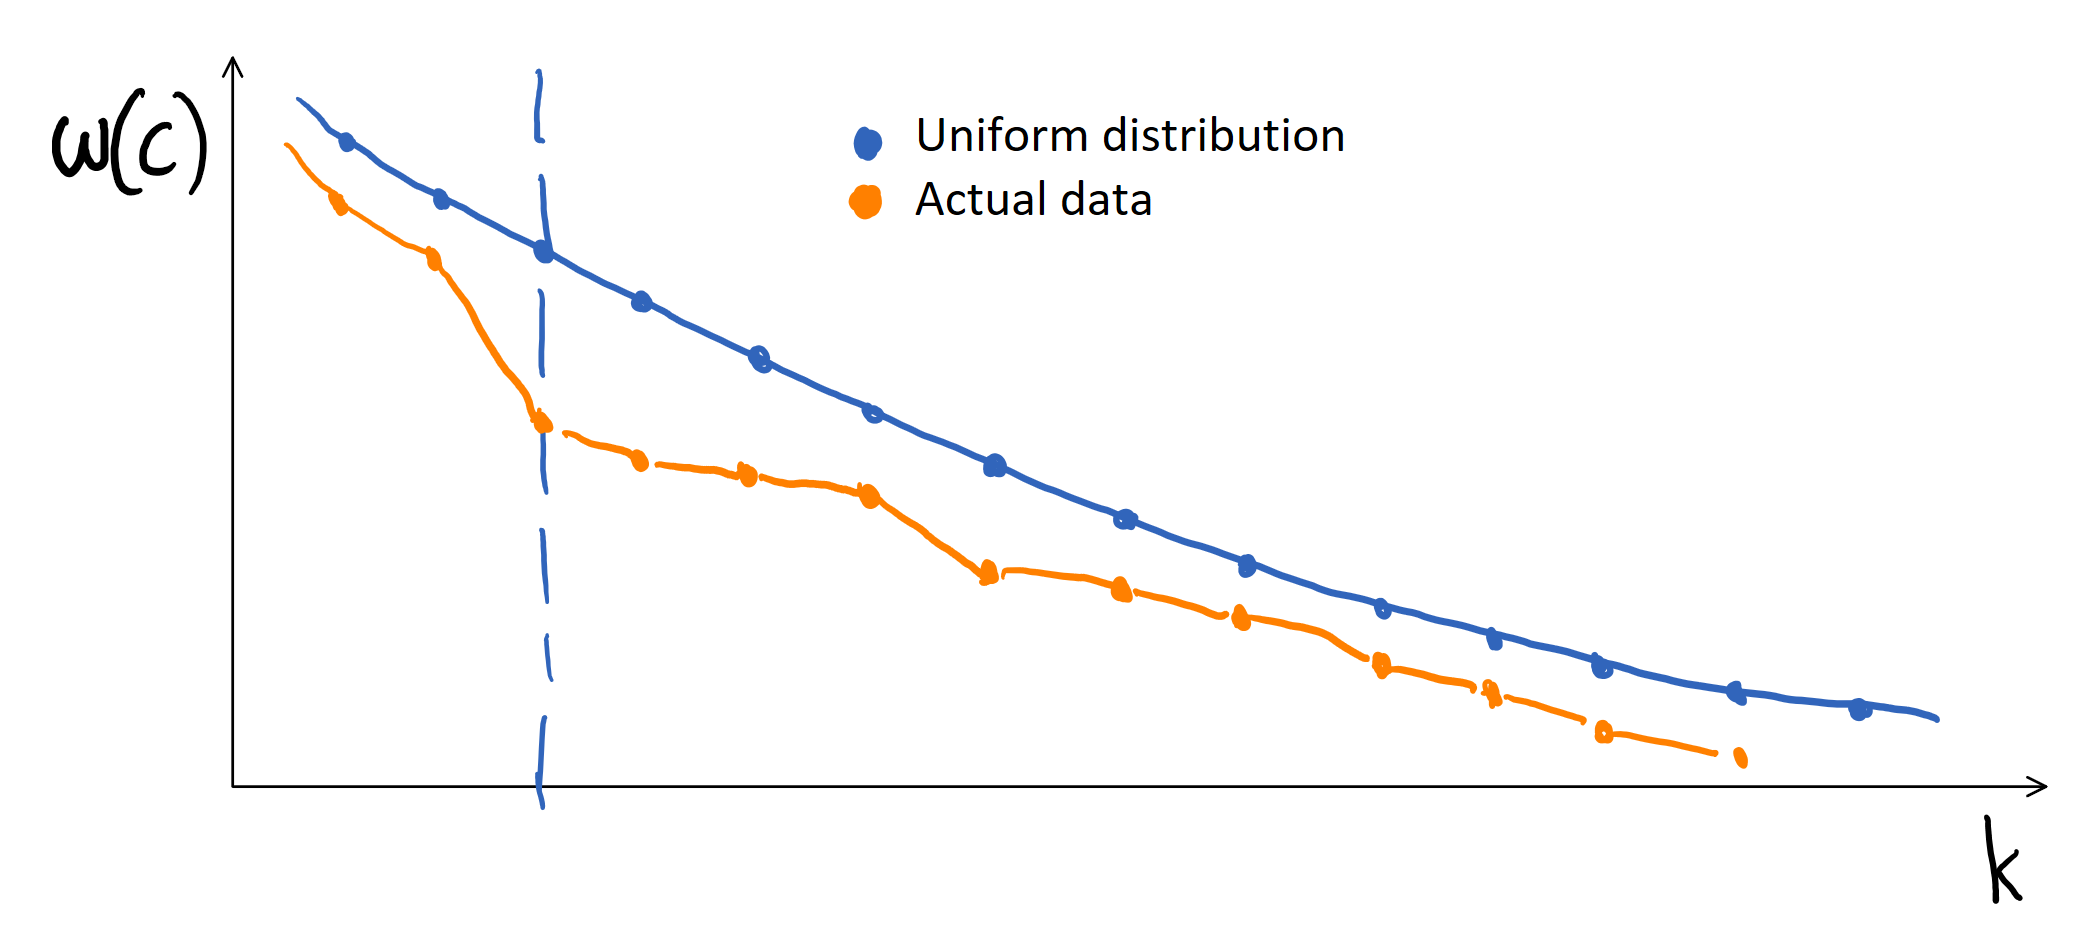
\includegraphics[width=\textwidth]{08-w_c-vs-w_prime_c}
   \caption{Approach 2: Relate change of $w(c)$ to change of $w'(c)$. Optimal \(K\) is where the gap between the two curves is largest (Proposed in \href{https://web.stanford.edu/~hastie/ElemStatLearn/}{TEoSL}).}
 	\end{minipage}
\end{figure}

\paragraph{Note:}
We have several options for clustering data. K-means and its variants are straight forward and easy to understand, but if the proper number of clusters is part of the unknowns, it may be a suboptimal choice.
One alternative is mean shift clustering. Here is the number of clusters determined implicitly by the kernel type and size plus the type of bump post process.
